\documentclass{beamer}

% \usepackage[lined,ruled]{algorithm2e}
\usepackage{subfigure}
\usepackage[english]{babel}
\usepackage[latin1]{inputenc}
\usepackage{times}
\usepackage[T1]{fontenc} 
\usepackage{color}

\usepackage{listings}
\usepackage{algorithm}
\usepackage{algpseudocode}
\usepackage{paralist}

% "define" Scala
\lstdefinelanguage{scala}{
  morekeywords={abstract,case,catch,class,def,%
    do,else,extends,false,final,finally,%
    for,if,implicit,import,match,mixin,%
    new,null,object,override,package,%
    private,protected,requires,return,sealed,%
    super,this,throw,trait,true,try,%
    type,val,var,while,with,yield, textFile, filter, cache, count,
    flatMap, map, reduceByKey, saveAsTextFile},
  otherkeywords={=>,<-,<\%,<:,>:,\#,@, <+=},
  sensitive=true,
  morecomment=[l]{//},
  morecomment=[n]{/*}{*/},
  morestring=[b]",
  morestring=[b]',
  morestring=[b]"""
}

\usepackage{color}
\definecolor{dkgreen}{rgb}{0,0.6,0}
\definecolor{gray}{rgb}{0.5,0.5,0.5}
\definecolor{mauve}{rgb}{0.58,0,0.82}
 
% Default settings for code listings
\lstset{frame=tb,
  language=scala,
  aboveskip=3mm,
  belowskip=3mm,
  showstringspaces=false,
  columns=flexible,
  basicstyle={\small\ttfamily},
  numbers=left,
  numberstyle=\tiny\color{gray},
  keywordstyle=\color{blue},
  commentstyle=\color{dkgreen},
  stringstyle=\color{mauve},
  frame=single,
  breaklines=true,
  breakatwhitespace=true
  tabsize=3
}


\usetheme[secheader]{Boadilla}
\usefonttheme[onlylarge]{structurebold}
\setbeamerfont*{frametitle}{size=\normalsize,series=\bfseries}
\setbeamertemplate{navigation symbols}{}
\setbeamertemplate{mini frames}[box]
\setbeamertemplate{sections/subsections in toc}[square]
\setbeamertemplate{blocks}[rounded][shadow=true]
\setbeamertemplate{bibliography item}[text]

\setbeamercolor{lightorange}{fg=black,bg=orange!40}
\setbeamercolor{lightblue}{fg=black,bg=blue!30}

\newenvironment{colorblock}[2]
{\setbeamercolor{item}{fg=#1,bg=#1}\begin{beamerboxesrounded}[upper=#1,lower=#2,shadow=true]}
  {\end{beamerboxesrounded}}



% Setup TikZ

\usepackage{tikz}
\usetikzlibrary{arrows}
\tikzstyle{block}=[draw opacity=0.7,line width=1.4cm]


%%%%%%%%%%%%%%%%%%%%%%%%%%%%%%%%%%%%%
%%%%%%%%%%%%%%%%%%%%%%%%%%%%%%%%%%%%%
%%%%%%%%%%%%%%%%%%%%%%%%%%%%%%%%%%%%%

\newtheorem{observation}[theorem]{Observation} 

%%%%%%%%%%%%%%%%%%%%%%%%%%%%%%%%%%%%%
%%%%%%%%%%%%%%%%%%%%%%%%%%%%%%%%%%%%%
%%%%%%%%%%%%%%%%%%%%%%%%%%%%%%%%%%%%%

\title{Algorithmic Machine Learning}
\subtitle{Introduction to the Course}
\author{Pietro Michiardi}
\institute{Eurecom}
\date


\begin{document}

\begin{frame}
  \titlepage
\end{frame}

%%%%%%%%%%%%%%%%%%%%%%%%%%%%%%%%%%%%%%%%%%%%%%%%%%%%%%%%%%
\section{Overview}

\begin{frame}
 \begin{colorblock}{blue}{lightblue}{ }
  \begin{center}
    \Huge \textbf{\texttt{Overview}}
  \end{center}
  \end{colorblock}
\end{frame}

\begin{frame}\frametitle{Objectives of the Course}
\begin{itemize}
	\item {\bf Gain hands-on experience on real-life Data Science projects}
	\item {\bf Use knowledge from ``theory'' courses and put them into practice}
	\item {\bf Use knowledge from ``systems'' courses} 
	\item {\bf Develop a methodology to address challenges such as:}
	\begin{itemize}
		\item Data preparation
		\item Data exploration
		\item Algorithm / model selection
		\item Experimental validation and evaluation
	\end{itemize}
\end{itemize}
\end{frame}

\begin{frame}\frametitle{Notebooks, not Lectures!}
\begin{itemize}
	\item {\bf Essentially, there will be no traditional lectures}
	\begin{itemize}
		\item Introduction to machine learning and advanced statistical inference
		\item Distributed systems and cloud computing
		\item Basic computer science skills are necessary
	\end{itemize}

	\item {\bf Notebooks}
	\begin{itemize}
		\item A self-contained studying and development environment
		\item Contains text, reference material, code, questions, graphs
		\item Each Data Science project will be your own project!
	\end{itemize}

	\item {\bf Publish your Notebooks!}
	\begin{itemize}
		\item Create a GitHub account and push your Notebooks there
		\item High-visibility of your own Data Science projects
		\item This is a sort of on-line CV
	\end{itemize}
\end{itemize}
\end{frame}

\begin{frame}\frametitle{Notebooks Content -- Schedule (1)}
\begin{itemize}
	\item {\bf Lab 1 [3/8/2017]}
	\begin{itemize}
		\item Introductory laboratory: getting familiar with Notebooks, Python, Numpy, Pandas, PySpark, Data Frames and more
	\end{itemize}

	\item {\bf Lab 2/3 [3/15/2017 - 3/22/2017]}
	\begin{itemize}
		\item Recommender Algorithms Project: work with real data from an Internet music streaming service, and recommend new music to users
	\end{itemize}

	\item {\bf Lab 4/5 [3/29/2017 - 4/5/2017]}
	\begin{itemize}
		\item Regression Algorithm Project: using random forests to predict airplane delays, using real data from the U.S. DoT
	\end{itemize}
\end{itemize}
\end{frame}

\begin{frame}\frametitle{Notebooks Content -- Schedule (2)}
\begin{itemize}
	\item {\bf Lab 5/6 [4/12/2017 - 4/26/2017]}
	\begin{itemize}
		\item Estimating Financial Risk through Monte Carlo Simulation
	\end{itemize}
	\item {\bf Lab 8/9 [5/3/2017 - 5/10/2017]}
	\begin{itemize}
		\item Clustering Algorithms Project: Anomaly Detection in Network Traffic with $k$-means Clustering
	\end{itemize}
	\item {\bf Industrial Lab [5/24/2017 - 5/31/2017]}
	\begin{itemize}
		\item Industrial Project from SAFRAN Analytics
	\end{itemize}
	\item {\bf Lab 10/11 [6/7/2017]}
	\begin{itemize}
		\item Analyzing Neuro-imaging Data with Thunder
	\end{itemize}
\end{itemize}
\end{frame}


\begin{frame}\frametitle{Industrial Notebooks}
\begin{itemize}
	\item {\bf Great opportunity to be exposed to real industrial problems}
	\begin{itemize}
		\item People from industry supervise the laboratory
		\item Main goal: hiring!
	\end{itemize}
	\item {\bf SAFRAN Analytics}
	\begin{itemize}
		\item \url{http://www.safran-group.com/}
		\item Distribute goodies
		\item Select best student(s) to participate to a SAFRAN event
	\end{itemize}
\end{itemize}
\end{frame}

\begin{frame}\frametitle{How to Be a Successful Student (1)}
\begin{itemize}
	\item {\bf Do not underestimate this course!}
	\begin{itemize}
		\item Be independent and dare to explore and expand your Notebooks
		\item Study or revise the theory: students are assumed to be comfortable with machine learning material, and to follow advanced statistical inference courses
		\item Follow links on the Notebooks. They contain reference material and research papers that: \emph{i)} provide the necessary background; \emph{ii)} offer starting point to improve algorithms
	\end{itemize}
	\item {\bf Is this a course about algorithm design?}
	\begin{itemize}
		\item Sort of: in many cases, Notebooks rely on standard libraries that offer a variety of machine learning algorithms implemented in an efficient way.
		\item Notebooks will illustrate the main algorithmic concepts behind a selection of tools available in such libraries
		\item Advanced (and optional) approaches to those proposed in the Notebooks are more than welcome!
	\end{itemize}
\end{itemize}
\end{frame}

\begin{frame}\frametitle{How to Be a Successful Student (2)}
\begin{itemize}
	\item {\bf Does this course make me a Data Scientist?}
	\begin{itemize}
		\item Sort of: it is the whole track that provides student with the necessary knowledge to start a Data Science career. This course aims at ``learning the hard way'' and put into practice theoretical concepts
	\end{itemize}
	\item {\bf Do I need to know how to program?}
	\begin{itemize}
		\item Yes, and this is mandatory
		\item We will focus on Python, but knowledge of additional languages is definitely a plus
	\end{itemize}
\end{itemize}
\end{frame}

\begin{frame}\frametitle{Grading}
\begin{itemize}
	\item {\bf Grading the laboratories / projects}
	\begin{itemize}
		\item Two-person groups are considered the norm
		\item Each Notebook/project is evaluated and graded
		\item Grading metrics
		\begin{itemize}
			\item Answer to Notebooks questions: this allows you to arrive at 10/20
			\item Depth of answers
			\item Originality of answers and approaches
			\item Additional points to innovative material in each Notebook
		\end{itemize}
	\end{itemize}
	\item {\bf Final exam}
	\begin{itemize}
		\item Depends on class behavior and performance
		\item Example: given a real world Data Science problem, outline an approach to address it, including:
		\begin{itemize}
			\item Relevant data exploration questions
			\item Relevant data cleaning warnings
			\item Model and algorithm selection
			\item Performance considerations
			\item Model validation
		\end{itemize}
	\end{itemize}
\end{itemize}
\end{frame}

\begin{frame}\frametitle{Useful References}
\begin{itemize}
	\item \emph{``An Introduction to Statistical Learning''}, by Gareth James, Daniela Witten, Trevor Hastie and Robert Tibshirani
	\item[] Available for download: \url{http://www-bcf.usc.edu/\~gareth/ISL/}

	\item \emph{``Advanced Analytics with Spark''}, by Sandy Ryza, Uri Laserson, Sean Owen, Josh Wills
	\item[] Available here: \url{http://shop.oreilly.com/product/0636920035091.do}, also available in the Library

	\item \emph{``Understanding Machine Learning: From Theory to Algorithms''}, by Shai Shalev-Shwartz and Shai Ben-David
	\item[] Available for download: \url{http://www.cs.huji.ac.il/~shais/UnderstandingMachineLearning/}
\end{itemize}
\end{frame}

%%%%%%%%%%%%%%%%%%%%%%%%%%%%%%%%%%%%%%%%%%%%%%%%%%%%%%%%%%

%%%%%%%%%%%%%%%%%%%%%%%%%%%%%%%%%%%%%%%%%%%%%%%%%%%%%%%%%%
\section{Infrastructure}

\begin{frame}
 \begin{colorblock}{blue}{lightblue}{ }
  \begin{center}
    \Huge \textbf{\texttt{Infrastructure}}
  \end{center}
  \end{colorblock}
\end{frame}

\begin{frame}\frametitle{EURECOM Cloud Computing Platform}
\begin{itemize}
	\item {\bf Private datacenter, hosted at Eurecom}
	\begin{itemize}
		\item Few hundres of server slots
		\item Pretty immutable network configuration
		\item No service level agreements
	\end{itemize}

	\item {\bf Cloud Computing Platform}
	\begin{itemize}
		\item Hybrid system: VM-based and container-based
		\item $O(1000)$ cores, $O(2 TB)$ RAM, $O(200 TB)$ storage
		\item No service level agreements
	\end{itemize}
\end{itemize}
\end{frame}

\begin{frame}\frametitle{Zoe Analytics}
\begin{itemize}
	\item {\bf Towards datacenter operating systems}
	\begin{itemize}
		\item Cluster scheduler, in the family of Borg, Mesos, and K8s
		\item Geared toward Analytics applications
		\item Scheduler and Resource allocator
		\item Based on Docker containers
	\end{itemize}

	\item {\bf Eurecom Open Source project}
	\begin{itemize}
		\item You can contribute!
		\item A lot of interest from many companies
		\item A platform for research
	\end{itemize}
\end{itemize}
\end{frame}

\begin{frame}\frametitle{Jupyter Notebooks}

	\begin{figure}
		
\includegraphics[width=0.45\linewidth]{figures/jupyter}
	\end{figure}

	\begin{colorblock}{blue}{lightblue}{ }
   The Jupyter Notebook is a web application that allows you to create and share documents that contain live code, equations, visualizations and explanatory text. Uses include: data cleaning and transformation, numerical simulation, statistical modeling, machine learning and much more.
   \end{colorblock}
\end{frame}

\begin{frame}\frametitle{Zoe Jupyter Applications}
	\begin{figure}
		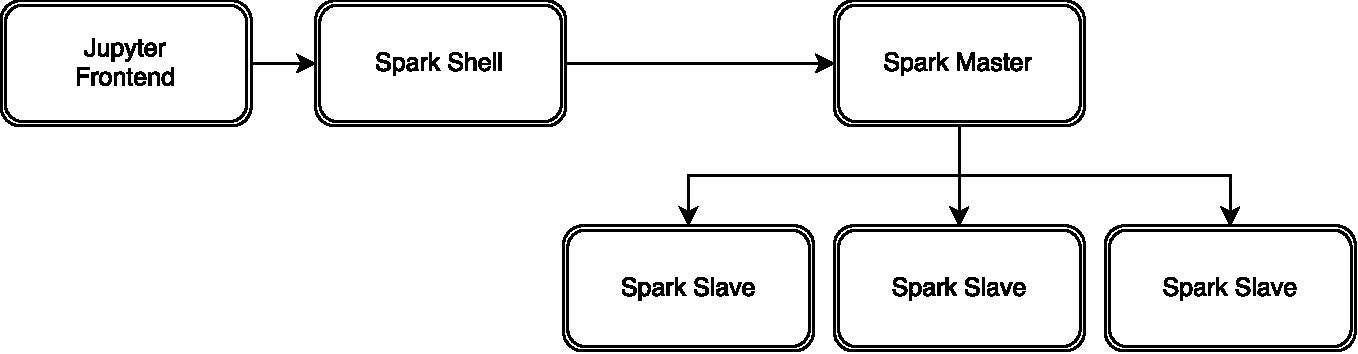
\includegraphics[scale=0.5]{figures/jupyter_app}
	\end{figure}
\end{frame}

\begin{frame}\frametitle{Working in the Lab}
\begin{itemize}
	\item {\bf Clone or Fork the AML-course repository}
	\item {\bf Working on your Notebook project}
	\begin{itemize}
		\item Upload your Notebook to the Zoe Jupyter application
		\item Work on your Notebook
		\item Download your Notebook as an iPython notebook
		\begin{itemize}
			\item This allows you to continue to work on your project during subsequent laboratory sessions, or eventually to work from home on a local installation
			\item It is strongly suggested to use GitHub!!
		\end{itemize}
	\end{itemize}
	\item {\bf Submitting your Notebook for evaluation}
	\begin{itemize}
		\item Download your Notebook as an html page
		\begin{itemize}
			\item Be careful! You need to save after you execute all cells!
		\end{itemize}
		\item Send by email the html version of the Notebook
	\end{itemize}
\end{itemize}
\end{frame}

%%%%%%%%%%%%%%%%%%%%%%%%%%%%%%%%%%%%%%%%%%%%%%%%%%%%%%%%%%


\end{document}
